\documentclass{article}

\usepackage{graphicx} % Allows including images
\usepackage{booktabs} % Allows the use of \toprule, \midrule and \bottomrule in tables
\usepackage{nicefrac}
%\usepackage{breqn}
\usepackage{algorithm}
\usepackage[noend]{algpseudocode}
\usepackage{amssymb}		% to get all AMS symbols
\usepackage{float}
\usepackage{cite} 
\usepackage{url}
\usepackage{amsmath,amsfonts,amsthm} % Math packages

\makeatletter
\def\BState{\State\hskip-\ALG@thistlm}
\makeatother

% --- CMDS --- (search for this header to jump to paper-specific
% commands)

\newcommand{\dd}[2]{\frac{\partial #1}{\partial #2}}
\newcommand{\Fnijk}[5]{{#1}^{(#2)}_{{#3}{#4}{#5}}}
\newcommand{\Fijk}[5]{{#1}_{{#2},{#3}{#4}{#5}}}
\newcommand{\Fn}[2]{\Fnijk{#1}{#2}{{}}{{}}{{}}}
\newcommand{\curl}[1]{\nabla \times {#1}}
\newcommand{\Enpo}{\Fn{E}{n+1}}
\newcommand{\Bnpo}{\Fn{B}{n+1}}
\newcommand{\En}{\Fn{E}{n}}
\newcommand{\Bn}{\Fn{B}{n}}
\newcommand{\dt}{\Delta t}
\newcommand{\iden}{\mathbf{I}}
\newcommand{\dx}{\Delta x}
\newcommand{\dy}{\Delta y}
\newcommand{\dz}{\Delta z}
\newcommand{\dxijk}[3]{\Delta x _{{#1}{#2}{#3}}}
\newcommand{\dyijk}[3]{\Delta y _{{#1}{#2}{#3}}}
\newcommand{\dzijk}[3]{\Delta z _{{#1}{#2}{#3}}}
\newcommand{\dxdual}{\Delta x_{i-\nicefrac{1}{2}jk}}
\newcommand{\dydual}{\Delta y_{ij-\nicefrac{1}{2}k}}
\newcommand{\dzdual}{\Delta z_{ijk-\nicefrac{1}{2}}}
\newcommand{\delxe}{(\curl{E})}

\begin{document}

\section{Problem Definition} 

\subsection{Discretization in Time}
Maxwells' equations ({\it sans} units) are:

\begin{align*}
  \dd{E}{t} &= \curl{B} \\
  \dd{B}{t} &= - \curl{E}
\end{align*}

We want to discretize these equations in time.
Given a fixed time step $\Delta t$, and temporal mesh $\Fn{t}{n}$, we do so by replacing
the time derivatives with a midpoint rule approximation and by replacing
the other quantities with an average of their values at the
endpoints.
In this way, we essentially replace each continuous
quantity with a second-order approximation of its value at the
midpoint of the interval $[\Fn{t}{n}, \Fn{t}{n+1}]$.
This discretization is known as the Crank-Nicholson time advance scheme.

Applying the discretization yields
\begin{align*}
  \Enpo - \En &= \frac{\dt}{2} ~\curl{ ( \Bnpo + \Bn ) } \\
  \Bnpo - \Bn &= - \frac{\dt}{2} ~\curl{ ( \Enpo + \En ) }
\end{align*}
Adding and subtracting a $\curl{\Fn{B}{n}}$ term and a $\curl{\Fn{E}{n}}$ term from the respective right-hand side of each of these equations yields
\begin{align*}
  \Enpo - \En &=  \dt ~\curl{\left( \Bn + \frac{1}{2} (\Bnpo -
      \Bn) \right)} \\
  \Bnpo - \Bn &= - \dt ~\curl{\left( \En + \frac{1}{2} (\Enpo -
      \En) \right)}
\end{align*}
If we now elect to substitute one of these equations (which one we
choose is arbitrary; let's go with the $B$ equation), we obtain:
\begin{align*}
  \Enpo - \En &= \dt ~\curl{\left( \Bn + \frac{\dt}{2}~\curl{\left( \En + \frac{1}{2} (\Enpo -
        \En) \right)} \right)} \\
\left(\iden + \frac{\dt^2}{4} ~\curl{(\curl)} \right) \Delta E &= \dt ~\curl{\Bn} -
\frac{\dt^2}{4} ~\curl{(\curl{\En})}
\end{align*}

Thus, advancing Maxwell's Equations one step forward in time using
this discretization involves applying the action of the inverse of the
operator
\begin{equation}
\mathbf{A} = \left(\iden + \frac{\dt^2}{4} \curl{(\curl)} \right)
\label{eq:1}
\end{equation}
with appropriate boundary conditions.

\subsection{Discretization in Space}

Now that we have identified the continuous form of the (spatial) operator
$\mathbf{A}$, we need to work on discretizing it.
The standard method for doing so was first developed by
Yee~\cite{yee1966numerical}.
In this method, the individual components of the electric and magnetic
fields are not known at all of the grid points; rather, they are known
at points offset from the grid points by half the grid spacing.
As shown in figure~\ref{fig:yeecell}, each grid point $r_{ijk}$ has associated
with it a rectangular prism with side lengths $\Delta x$, $\Delta y$, and $\Delta
z$, and its back lower left corner located at $r_{ijk}$.
The components of the electric field are displaced so that they are located
at the midpoints of the {\em edges} of the cube {\em parallel} to them and
containing $r_{ijk}$.
components of the magnetic field are displaced so that they are
located at the centers of the {\em faces} of the cube {\em normal} to
them and containing $r_{ijk}$

\begin{figure}[htbp]
  \centering
  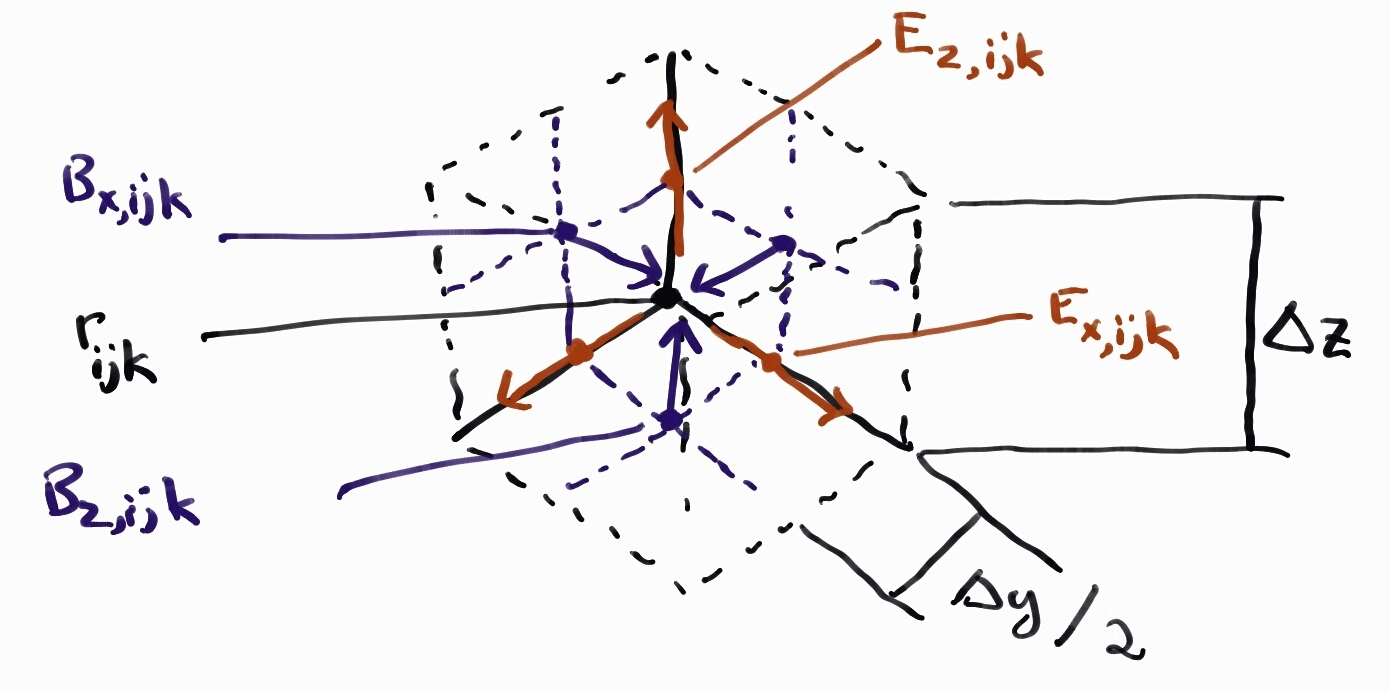
\includegraphics[width=0.5\textwidth]{YeeCellDiagram}
  \caption{Yee Grid Cell}
  \label{fig:yeecell}
\end{figure}

Locating the fields at these points is convenient for computing
curls.  The $x$ component of $\curl{E}$ is required to update $B_x$.
Figure~\ref{fig:yeecurl} illustrates the field components required to
calculate $(\curl{E})_x$ on the Yee mesh.  Stokes' Theorem suggests
that we would like to do a line integral around the edge of our face
and divide by the area, like so:

\begin{equation}
(\curl{E})_x = \frac{ \dz (\Fijk{E}{z}{i}{j+1}{k} -
  \Fijk{E}{z}{i}{j}{k}) - \dy (\Fijk{E}{y}{i}{j}{k+1} -
  \Fijk{E}{y}{i}{j}{k}) }{\dy \dz}\label{eq:2}
\end{equation}

\begin{figure}[htbp]
  \centering
  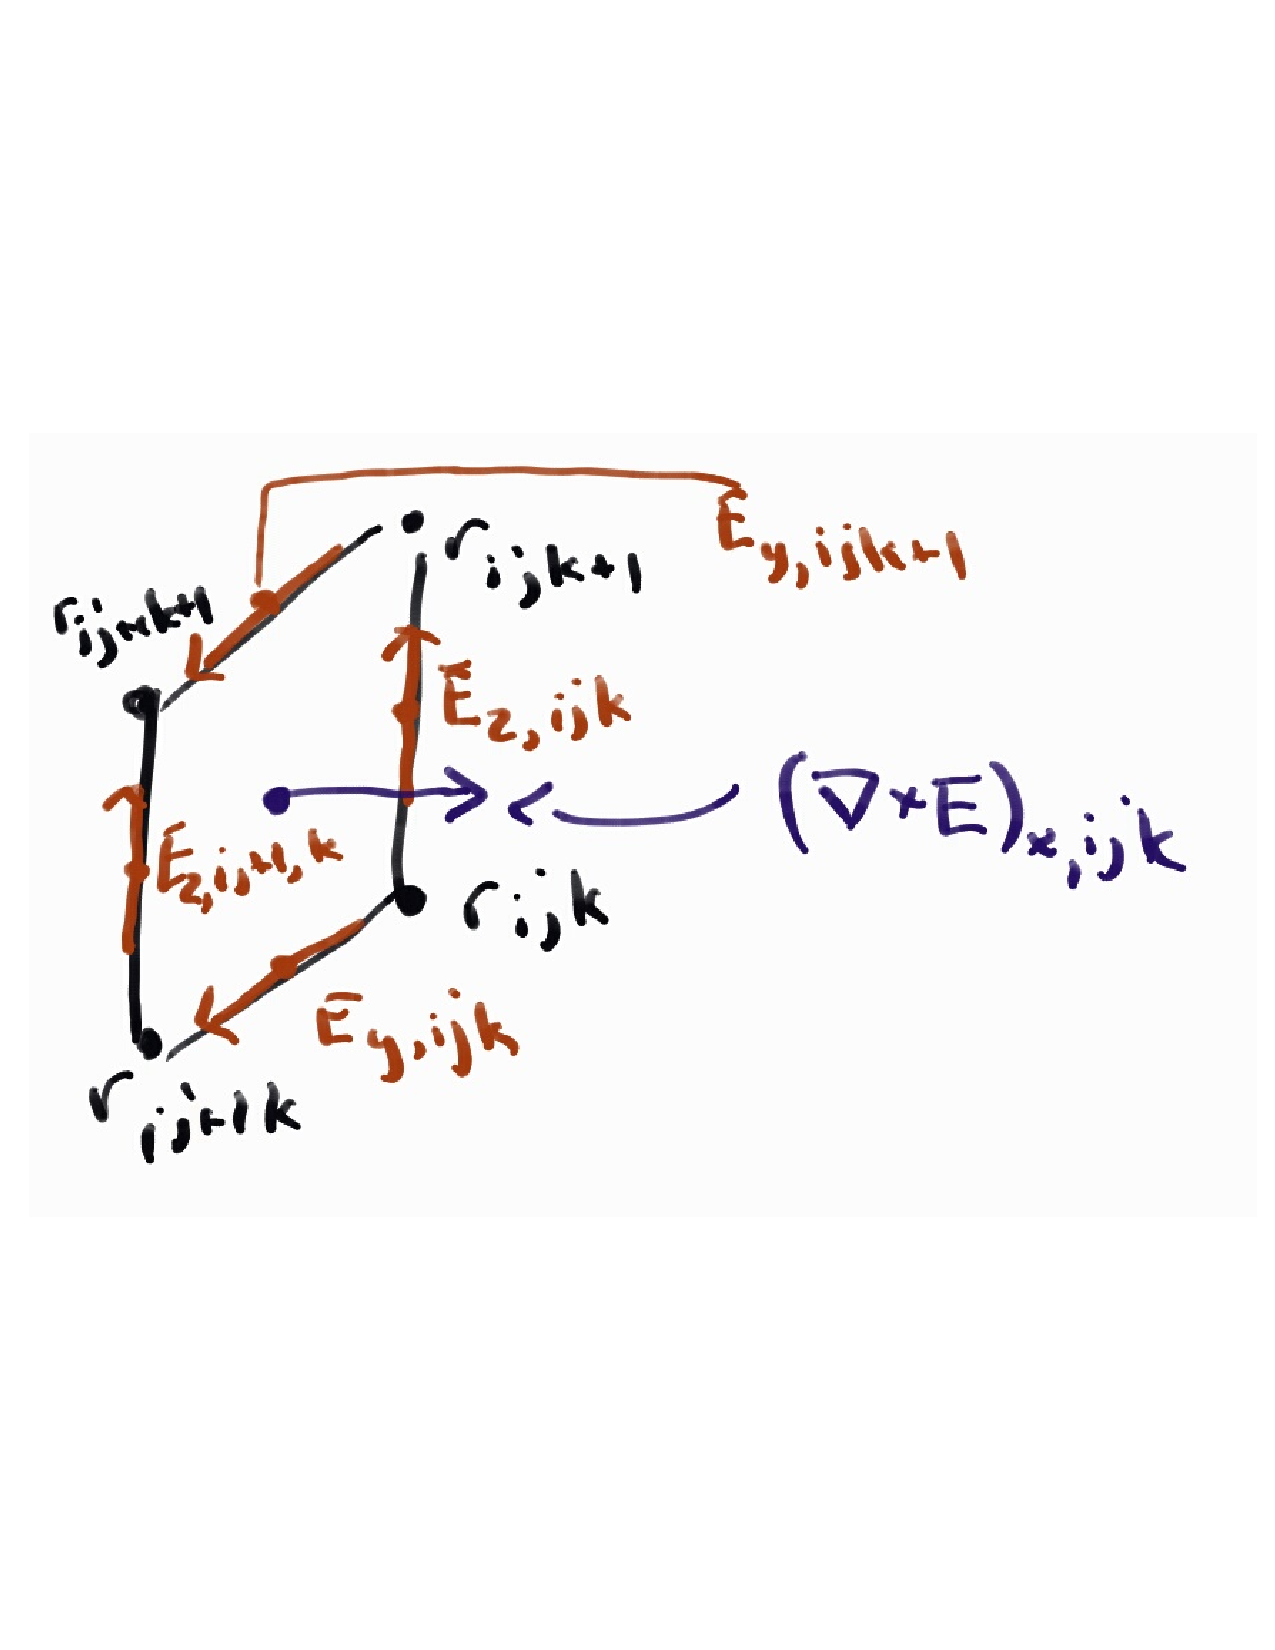
\includegraphics[width=0.5\textwidth]{CurlDiagram.pdf}
  \caption{Calculating Curl on Yee Mesh}
  \label{fig:yeecurl}
\end{figure}

The procedure for determining $\curl{B}$ is similar; the edge of
each prism is surrounded by four faces whose centers describe a
rectangle (part of what is often referred to as ``the Dual Grid'') on
which we can use Stokes' Theorem.  One subtlety: with the indexing
convention shown, the edges bordering a face associated with $r_i$ are associated with $r_i$ and
$r_{i+1}$, but the {\em faces} bordering an {\em edge} associated with
$r_i$ are associated with $r_i$ and $r_{i-1}$, so the expression for
the curl will have different indices.

We  also see here that curl is an
operator that transforms ``face quantities'' into ``edge quantities''
and {\it vice versa} on the Yee mesh.  It follows, since $E$ is an
edge quantity, that $\curl{(\curl{E})}$ is also an edge quantity.  Let
us move towards an expression for it.  Since our Yee cells might all
be different sizes, we record within each its size lengths $\dx_{ijk}$.  If we define
$\dz_{ijk-\nicefrac{1}{2}} = \frac{1}{2} (\dz_{ijk-1} + \dz_{ijk})$,
then a discretized expression for $\curl{\delxe}$ is

\begin{multline}
  (\curl{ \delxe })_x = \\ \frac{\dz_{ijk-\nicefrac{1}{2}}
    (\Fijk{\delxe}{z}{i}{j}{k} - \Fijk{\delxe}{z}{i}{j-1}{k}) -
    \dy_{ij-\nicefrac{1}{2}k} (\Fijk{\delxe}{y}{i}{j}{k} -
    \Fijk{\delxe}{y}{i}{j}{k-1}) }{\dy_{ij-\nicefrac{1}{2}k} \dz_{ijk-\nicefrac{1}{2}} }\label{eq:3}
\end{multline}

Substituting the expression~\ref{eq:1} for the components of $\delxe$
(appropriately modified for each component) into equation~\ref{eq:3}
yields the following result:

\begin{multline}
  \label{eq:4}
  (\curl{ \delxe})_x = \\
  - \frac{1}{\dydual}
  \left( \frac{  \Fijk{E}{x}{i}{j+1}{k}  - \Fijk{E}{x}{i}{j}{k}}
    {\dyijk{i}{j}{k}}
    - \frac{  \Fijk{E}{x}{i}{j}{k}  - \Fijk{E}{x}{i}{j-1}{k}}
    {\dyijk{i}{j-1}{k}} \right) \\
  - \frac{1}{\dzdual}
  \left( \frac{  \Fijk{E}{x}{i}{j}{k+1}  - \Fijk{E}{x}{i}{j}{k}}
    {\dzijk{i}{j}{k}}
    - \frac{  \Fijk{E}{x}{i}{j}{k}  - \Fijk{E}{x}{i}{j}{k-1}}
    {\dzijk{i}{j-1}{k}} \right) \\
  +
  \left( \frac{\Fijk{E}{y}{i+1}{j}{k} - \Fijk{E}{y}{i+1}{j-1}{k}}
    {\dydual \dxijk{i+1}{j}{k}}
    - \frac{\Fijk{E}{y}{i}{j}{k} - \Fijk{E}{y}{i}{j-1}{k}}
    {\dydual \dxijk{i}{j}{k}} \right) \\
+
  \left( \frac{\Fijk{E}{z}{i+1}{j}{k} - \Fijk{E}{y}{i+1}{j}{k-1}}
    {\dzdual \dxijk{i+1}{j}{k}}
    - \frac{\Fijk{E}{y}{i}{j}{k} - \Fijk{E}{y}{i}{}{k-1}}
    {\dzdual \dxijk{i}{j}{k}} \right)
\end{multline}
We can add zero to the right hand side of this equation in an
instructive manner:

\begin{multline}
  \label{eq:5}
  (\curl{ \delxe})_x = \\
  - \frac{1}{\dydual}
  \left( \frac{  \Fijk{E}{x}{i}{j+1}{k}  - \Fijk{E}{x}{i}{j}{k}}
    {\dyijk{i}{j}{k}}
    - \frac{  \Fijk{E}{x}{i}{j}{k}  - \Fijk{E}{x}{i}{j-1}{k}}
    {\dyijk{i}{j-1}{k}} \right) \\
  - \frac{1}{\dzdual}
  \left( \frac{  \Fijk{E}{x}{i}{j}{k+1}  - \Fijk{E}{x}{i}{j}{k}}
    {\dzijk{i}{j}{k}}
    - \frac{  \Fijk{E}{x}{i}{j}{k}  - \Fijk{E}{x}{i}{j}{k-1}}
    {\dzijk{i}{j-1}{k}} \right) \\
  - \frac{1}{\dxdual}
  \left( \frac{  \Fijk{E}{x}{i+1}{j}{k}  - \Fijk{E}{x}{i}{j}{k}}
    {\dxijk{i}{j}{k}}
    - \frac{  \Fijk{E}{x}{i}{j}{k}  - \Fijk{E}{x}{i-1}{j}{k}}
    {\dxijk{i-1}{j}{k}} \right) \\
  +
  \left( \frac{\Fijk{E}{y}{i+1}{j}{k} - \Fijk{E}{y}{i+1}{j-1}{k}}
    {\dydual \dxijk{i+1}{j}{k}}
    - \frac{\Fijk{E}{y}{i}{j}{k} - \Fijk{E}{y}{i}{j-1}{k}}
    {\dydual \dxijk{i}{j}{k}} \right) \\
  + \left( \frac{\Fijk{E}{z}{i+1}{j}{k} - \Fijk{E}{y}{i+1}{j}{k-1}}
    {\dzdual \dxijk{i+1}{j}{k}}
    - \frac{\Fijk{E}{y}{i}{j}{k} - \Fijk{E}{y}{i}{j}{k-1}}
    {\dzdual \dxijk{i}{j}{k}} \right) \\
  + \left( \frac{\Fijk{E}{z}{i+1}{j}{k} - \Fijk{E}{y}{i}{j}{k}}
    {\dzdual \dxijk{i+1}{j}{k}}
    - \frac{\Fijk{E}{y}{i}{j}{k} - \Fijk{E}{y}{i-1}{j}{k}}
    {\dzdual \dxijk{i}{j}{k}} \right)
\end{multline}

Squinting hard and looking at equation~\ref{eq:5}, you should be able
to convince yourself that it is at least a plausible discretization of
the vector identity $\curl{ \delxe} = -\nabla^2 E + \nabla (\nabla
\cdot E)$ (A few words on the quality of this discretization will
follow).  In a charge-free region, $\nabla \cdot E = 0$ (an equation
which the uniform-grid Crank-Nicholson Yee time advance can be shown
to preserve in discrete form), allowing us to eliminate the last three
terms of the equation above, and reducing our equation to 

\begin{multline}
  \label{eq:6}
  (\curl{ \delxe})_x = \\
  - \frac{1}{\dydual}
  \left( \frac{  \Fijk{E}{x}{i}{j+1}{k}  - \Fijk{E}{x}{i}{j}{k}}
    {\dyijk{i}{j}{k}}
    - \frac{  \Fijk{E}{x}{i}{j}{k}  - \Fijk{E}{x}{i}{j-1}{k}}
    {\dyijk{i}{j-1}{k}} \right) \\
  - \frac{1}{\dzdual}
  \left( \frac{  \Fijk{E}{x}{i}{j}{k+1}  - \Fijk{E}{x}{i}{j}{k}}
    {\dzijk{i}{j}{k}}
    - \frac{  \Fijk{E}{x}{i}{j}{k}  - \Fijk{E}{x}{i}{j}{k-1}}
    {\dzijk{i}{j-1}{k}} \right) \\
  - \frac{1}{\dxdual}
  \left( \frac{  \Fijk{E}{x}{i+1}{j}{k}  - \Fijk{E}{x}{i}{j}{k}}
    {\dxijk{i}{j}{k}}
    - \frac{  \Fijk{E}{x}{i}{j}{k}  - \Fijk{E}{x}{i-1}{j}{k}}
    {\dxijk{i-1}{j}{k}} \right)
\end{multline}

Equation~\ref{eq:5} gives us a 7-point stencil defining a matrix for
$\curl{\delxe}$, and hence the operator given in equation~\ref{eq:1}
in a charge-free region.  Furthermore, the
inhomogoneous Gauss's Law $\nabla \cdot E = \frac{\rho}{\epsilon_0}$
allows us to move the $\nabla(\nabla \cdot E)$ term to the right hand
side without solving for it explicitly, so this process is applicable
to problems with charges and currents as well.

The matrix defined here is block-banded with seven bands, and is not
symmetric.

\section{Multigrid for solving Maxwell's Equations}

	In this section, we develope an algorithm for solving the discretization of Maxwell's equation given in the previous section.  The goal is for the algorithm to perform well independent of the size of the problem. This algorithm will be an algebraic multigrid method.  We begin by describing a general multigrid method, and then introduce the elements of multigrid specfic to this problem.

\subsection{General Multigrid}

Multigrid methods are among the most efficient algorithms to solve linear systems of the form $Ax=b$.  These systems arise often in applications varying from numerically solving PDEs to graph analysis.  The most important aspect of a multigrid method is a hierarchy of grid levels, $\{\Omega_i\}_{i=1}^L$ that each have a different resolution.  Corrections applied on different grid levels act in a complementary manner to accelerate the convergence of the solutions.  Often a smoother such as weighted Jacobi or Gauss-Siedel is applied on the finest grid, $\Omega_1$, to eliminate the high energy error modes. The resulting smooth residual in the restricted to a coarser grid, $\Omega_2$, to be solved for exactly.  Once calculated, the coarse residual is interpolated back to the fine grid, where it is added to the fine grid approximation. In this way, the high energy residuals are smoothed away on the fine grid, and low energy residuals are accounted for using a coarse grid correction scheme.

In practice, the coarse grid problem is not solved directly, but rather a multigrid scheme is used again.  The coarse grid ($\Omega_2$) approximation is smoothed and then restricted to an even coarser grid, $\Omega_3$.  This process is repeated iteratively until a sufficiently coarse grid, $\Omega_L$, is reached where the linear system can be solved directly.  Once the coarsest grid is solved for, the solution is interpolated back up to the finer grids ($\Omega_{L-1}, \Omega_{L-2},...$) all the way back to the orignial fine grid.  In practice,a post-smoothing is applied after each coarse grid correction step, in-case new high energy errors are introduced by the interpolation operator.  Often we refer to this recursive algorithm type as a $V(\mu_1,\mu_2)$ cycle. The $V$ is in reference to the shape of the diagram describing the manner in which the grid hierarchy is travelled.  $\mu_1$ and $\mu_2$ refer to the number of pre and post smoothing iterations applied, respectively.

There are other more complicated recursive patterns for multigrid methods, such as a $W$ cycle which often lead to faster convergence rates, but higher code complexity and computational cost.  Regardless of the recursive pattern, there are essentially two operators on each grid that fully define a multigrid method. First, you need a  relaxation operator on each grid level, $\{R_1,R_2,...,R_L\}$. Second, you need an inter-grid transfer operators, $\{P_1,P_2,...,P_L\}$.  Note that $P_k$ is an interpolation operator to move from grid $\Omega_k$ to the finer grid $\Omega_{k-1}$.  We will use the notation $R_k$ to denote the restriction operator that restricts vectors from grid $\Omega_k$ to the coarser grid $\Omega_{k+1}$.  The following figure gives the outline of a generic $V$ cycle.

\begin{algorithm}
\caption{Standard Multigrid V-cycle}\label{euclid}
\begin{algorithmic}[1]
\Procedure{V}{$A_k,b_k,u_k,k$}
\State $u_k \gets R_k(A_k,b_k,u_k)$
\If {$k \neq L$}
\State $r_k \gets b_k - A_k u_k$
\State $A_{k+1} \gets  P_{k+1}^T A_k P_{k+1}$
\State $u_{k+1} \gets 0$
\State $V(A_{k+1},P_{k+1}^T r_k,u_{k+1},k+1)$
\State $u_k \gets u_k + P_{k+1} u_{k+1}$
\State $u_k \gets R_k(A_k,b_k,u_k)$
\EndIf
\EndProcedure
\end{algorithmic}
\end{algorithm}

\newpage

\subsection{Geometric Multigrid and Maxwell's Equations}

Let us consider the simple test case of solving Poisson's equation on a 1D domain.

\begin{equation}
\label{eq:7}
 \frac{d^2u}{dx^2} = f(x), \;\;\;\;  0 \leq x \leq 1 
\end{equation}

In this case, the operator $A_k$ just comes from discretizing the domain and approximating the Laplacian on this grid with some finite difference method. To attain the next coarsest grid's operator, $A_{k+1}$, one merely needs to re-discretize the domain with a larger mesh spacing and again approximate the Laplacian operator using a finite difference method. The interpolation operator, $P_k$, is usually choosen simply to be linear interpolation.  Restriction operators, $R_k$, are just defined as the transpose of $P_k$ multiplied by a scaling constant to preserve magnitudes of vectors.

When the system to be solved is based on a physical model, like in the Poisson case, the algorithm used is referred to as \textit{Geometric Multigrid}.  Often these are cases involving discretizations of PDEs.  If the problem has a geometric nature, then defining the coarse grid operators $A_k$ just entails re-discretizing your domain with a coarser mesh, and then re-discretizing your PDE on this mesh.  This means you need to know something about the geometry of your problem to utilize geometric multigrid methods.  Geometric multigrid is the most intuitive form of multigrid. However, it is restrictive in that the code requires a predetermined mesh hierarchy.  Examples of Geometric Multigrid implementations can be seen in ~\cite{briggs2000multigrid} and ~\cite{hackbusch1985multi}.


If we return to the discretization of Maxwell's Equations developed in section 1, we recall that we rewrite the continuous equation

\begin{equation}
\label{eq:8}
\curl{\curl{E}} + \sigma E = f 
\end{equation}

as
\begin{equation}
\label{eq:9}
K_1^{(e)} e_1 = f_1
\end{equation}

Where $e_1$ is the vector of electric field values along edges, and $K_1 = S_1 + M_1$.  $S_1$ is the discrete \textit{curl,curl} operator, and $M_1$ is the discrete form of the second term in equation~\ref{eq:8}.  Upon inspection of $S_1$ we notice some curious behavior. For any scalar valued function, $\phi$, it is true that 

\begin{equation}
\label{eq:10}
\curl{(\nabla \phi)} = 0
\end{equation}

 If  $\curl{(\nabla \phi)} = 0$, then we know that the gradients of scalar functions, $\nabla\phi$, live in kernel of the \textit{curl,curl} operator. Let us denote the discrete gradient operator as $T_1$.  It is a simple matrix to create. Every row contains at most two non-zeros with values of $+1$ or $-1$ representing connections edges in the nodal graph. Now we can enforce equation \ref{eq:10} with the following discrete equation

$$S_1T_1 = \bf{0}$$

Low energy functions have low energy gradients, and high energy functions have high energy gradients.  This means that there are both smooth and oscillatory functions in the kernel of $K_1$. The crux of any successful method is to adapt to the consequences of equation~\ref{eq:10}.  Hitmair developes an \textit{h} independent geometric algorithm in~\cite{hiptmair1998multigrid}.  For the remainder of this paper, we will steer away from geometric multigrid algorithms in favor of algebraic methods.

\subsection{Algebraic Multigrid} 

Consider the problem of solving the linear system $Ax = b$.  In physics and engineering, it is often the case the these systems arize from models of physical phenomena or PDEs.  In this case, we have already discussed the power of geometric multigrid.  However, it can often be the case that the system $Ax=b$ does not represent a physical model at all, or that the model has a very irregular geometry.  If the geometry is difficult, the mesh is irregular, or the problem is non-physical, then we can run into problems when implementing geometric multigrid as discussed in previous sections.  

In this case, we use a class of methods known as \textit{Algebraic Multigrid} (AMG).  In AMG algorithms we still use a hierarchy of complementary linear systems to accelerate the convergence of the solution on the finest grid. We still have the same concept of fine grid relaxation and coarse grid correction.  The difference between AMG and geometric multigrid is that in AMG all grid transfer operators and coarse grid operators are derived directly from the entries in the $A$ matrix.  In geometric settings, the $A$ matrix is formed from a re-discretization of the domain, whereas in AMG the new $A$ matrix is defined purely by the Galerkin product

\begin{equation}
\label{eq:11}
A_{k+1} = P_k^T A_k P_k
\end{equation}
and the projection operator is choosen carefully to yield desired error damping characteristics.


\subsection{Smoothed Aggregation} 

The algorithm presented in \cite{ Hu2006} showcases an algebraic multigrid (AMG) approach to solving Maxwell's equations which is only slightly dependent on $h$, the discretization step size. The crux of this algorithm is the choice of interpolation (or prolongation) operators, $P_k$. More specifically, the method is to smooth the prolongator, along with the idea of aggregation of points into what are called {\it supernodes}, to achieve an algorithm nearing $h$-independence. For these reasons, this technique is referred to as {\it smoothed aggregation}. A smoothed aggregation multigrid algorithm, and convergence theory concerning said algorithm, is presented in \cite{Brezina2000}. The algorithm and some salient results from that paper are repeated here. 

We are interested in solving
\[
A{\vec x} = {\vec b}
\]
\noindent with a multilevel technique, where $A$ is a matrix representing the discretization of some differential operator (in this case the curl curl relation presented in the previous section). Multigrid with smoothed aggregation is equivalent to standard multigrid, save the difference in interpolation operators. Here we use a smoothing operator $\Sigma_{k}$ on an algebraically determined prolongation operator $P_{k}$ such that
\[
P_{k}:\mathbb{R}^{n_{k+1}}\rightarrow\mathbb{R}^{n_{k}},
\]
\noindent where $k=1,...,L$-1 and $L$ is the number of levels in the scheme. $k=1$ represents the finest grid. This is called the {\it tentative prolongator operator}, and it is of full rank. We note that $\Sigma_{k}$ is a smoothing matrix constructed from the information within $A$ such that $\Sigma_{k}:\mathbb{R}^{n_{k}}\rightarrow\mathbb{R}^{n_{k}}$. Then the hierarchy of coarse level matrices is given by the Galerkin relation after smoothing $P_k$
\[
A_{k+1} = \left(\Sigma_{k}P_{k}\right)^{T}A_k~ (\Sigma_{k}P_{k}),
\]
\noindent The multigrid algorithm used is essentially a V-cycle. The algebraic aspect of the algorithm rests in the construction of the prolongator operator. 

The tentative prolongator is constructed using the aforementioned supernodes concept in the following way: the degrees of freedom on each level are organized into ``small, disjoint clusters", or aggregates. Once the hierarchy of aggregates is known, we need only the matrix $B^{1}$. The dimensions of this matrix are $n_{1}\times$$r$, where $r$ is the number of aggregates on the $k^{th}$ level. The range of $B^{1}$ indicates the vectors on the finest grid which should be ``exactly representable", in the sense that rng$\left(B^{1}\right)\subset$ rng$\left(P^{1}_{k}\right)$, where $P^{1}_{k}$ is the {\it composite tentative operator}, given by
\[
P^{1}_{k} = P_{2}...P_{k-1},
\]
\noindent with $P_{1}^{1}=I$. $B^{1}$ is typically chosen to be a generator of so-called {\it zero energy modes}. In the Finite Element context, this is the kernel of the stiffness matrix from a Finite Element model {\it sans} essential boundary conditions. These generators are available in most Finite Element packages. 

The aforementioned property of rng$\left(B^{1}\right)$ is enforced by simultaneously creating the prolongator $P_{k}$ along with the $n_{k+1}\times$$r$ matrix $B^{k+1}$ such that
\[
P_{k}B^{k+1} = B^{k}.
\]
\noindent This relation is enforced in an aggregate-by-aggregate fashion. The construction algorithm for the prolongator is now presented for a given system of aggregates $\{\mathcal{A}_{i}^{k}\}_{i=1}^{N_{k}}$, where $N_{k}$ is the number of aggregates on the $k^{th}$ level.
\paragraph{{\bf Algorithm.}} {\it For the system of aggregates} $\{\mathcal{A}_{i}^{k}\}_{i=1}^{N_{k}}$ {\it and the} $n_{k}\times$$r$ {\it matrix} $B^{k}$ {\it satisfying} $P_{k}^{1}B^{k}=B^{1}$,{\it construct a prolongator} $P_{k}$, {\it along with another matrix} $B^{k+1}$ {\it such that} $P_{k}B^{k+1}=B^{k}$ {\it and supernodes on level} $k+1$ {\it in the following manner}:
\begin{enumerate}
\item Let $d_{i}$ be the degrees of freedom for the $i^{th}$ aggregate $\mathcal{A}_{i}^{k}$. Affect the partition of $B^{k}$ into blocks $B_{i}^{k}$ of size $d_{i}\times$$r$ for $i=1,...,N_{k}$, each corresponding to the set of degrees of freedom on the $i^{th}$ aggregate.
\item $QR$-decompose $B_{i}^{k}$=$Q_{i}^{k}R_{i}^{k}$.
\item Create tentative prolongator $P_{k}=$diag$\left(Q_{1}^{k},...,Q_{N_{k}}^{k}\right)$, and set
\[ B^{k+1}=\left( \begin{array}{c}
R_{1}^{k}\\
R_{2}^{k}\\
...\\
R_{N_{k}}^{k}\end{array} \right).\] 
\end{enumerate}
\noindent Coarsening on each aggregate $\mathcal{A}_{i}^{k}$ results in $r$ degrees of freedom on the coarse level. These degrees of freedom define the $i^{th}$ coarse-level supernode.

This algorithm produces the tentative prolongator algebraically. When this strategy is applied to solving Maxwell's Equations, this prolongator is updated by effectively lowering its energy via a damped Jacobi iteration
\[
P'_{k} = \left(I-\gamma D^{-1}A\right)P_{k},
\]
\noindent where $P_{k}$ is the tentative prolongator, $\gamma$ is the damping parameter, and $D=$diag$\left(A\right)$ \cite{Hu2006}. The prolongator is hit with the smoothing matrix $\Sigma_{k}$ before using it in the interpolation step.

\subsection{Smoothed Aggregation AMG on Maxwell's Equations}

While a few successful geometric multigrid methods exist for solving Maxwell's Equations, very few AMG methods exist.  Reitzinger and Schoberl were the first to develope an AMG method~\cite{reitzinger2002algebraic}. In their approach, they use two grid hierarchies to achieve accurate results.  One hierarchy is for nodal values and the second hierarchy is for edge values.  The key goal is to retain the representation of a discrete gradient on coarse meshes, and maintain its relationship to the discrete \textit{(curl,curl)} operator.  

The main hierarchy is for edge values, and coarsens the space on which the discrete Maxwell's Equations (\ref{eq:9}) live. The secondary hierarchy of nodes is just needed to setup the main hierarchy. Specifically, it is used in computing $P_k^{(e)}$.  Note that now we have operators for both hierarchies. The superscript $(e)$ represents edge items and the $(n)$ represents nodal items. 



To begin we construct the auxiliary hierarchy. We discretize the following PDE 

\begin{equation}

\int_{\Omega} \sigma u \dot v + \int_{\Omega} \nabla u \dot \nabla v = 0

\end{equation}


to achieve a nodal operator $K_1^{(n)}$




For the edge hierarchy, given a projection operator, $P_k^{(e)}$ the new edge matrix is simply calculated using the Galerkin Product
\[
K_{k+1}^{(e)} = (P_k^{(e)})^T K_k^{(e)} P_k^{(e)}
\]






\subsection{Improving the Prolongation Operator}
The novelty of the algorithm in \cite{Hu2006} is a proverbial ``beefing up" of the tentative prolongator calculated via smoothed aggregation. That is, consider a prolongation operator of the form
\[
P'_{k} = \left(I-\alpha D_{S,k}^{-1}S_{k}+\beta T_{k}D_{T,k}^{-1}T_{k}^{T}{\hat M}_{k}\right)P_{k},
\]
\noindent where $S_{k}$ is the discrete {\it curl, curl} on the $k^{th}$ level, and $T_{k}$ is the discretized gradient on the same level. The $D$ matrices are the diagonals of the matrices corresponding to their subscripts. ${\hat M}_{k}$ is the approximation of the mass matrix $M_{k}$, obtained by lumping the off-diagonal elements of $M_{k}$ into the diagonal terms. $\alpha$ and $\beta$ are damping parameters, chosen such that they optimize energy properties as per the theory presented in \cite{Brezina2000}:
\begin{align*}
  \alpha &= \frac{4}{3}\rho\left(D_{S,k}^{-1}S_{k}\right)^{-1},\\
  \beta &= \frac{4}{3}\rho\left(D_{T,k}^{-1}T_{k}^{T}M_{k}T_{k}\right)^{-1}.
\end{align*}


\section{Trilinos}


\bibliographystyle{plain}
\bibliography{EandMDescription}

\end{document} 